\section{An�lisis}\label{sec:analysis}

\subsection{\label{subsec:analisis1}}

Las figuras~\ref{fig:S1L1},~\ref{fig:S1L2} y~\ref{fig:S1L3} representan la relaci�n $\Delta V$ frente a $I$ para el primer cable
para las 3 longitudes.

De igual modo, las figuras~\ref{fig:S2L1},~\ref{fig:S2L2} y~\ref{fig:S2L3} corresponden al segundo cable y
las~\ref{fig:S3L1},~\ref{fig:S3L2} y~\ref{fig:S3L3}
al tercero.

\begin{figure}[h!]
    \begin{center}
        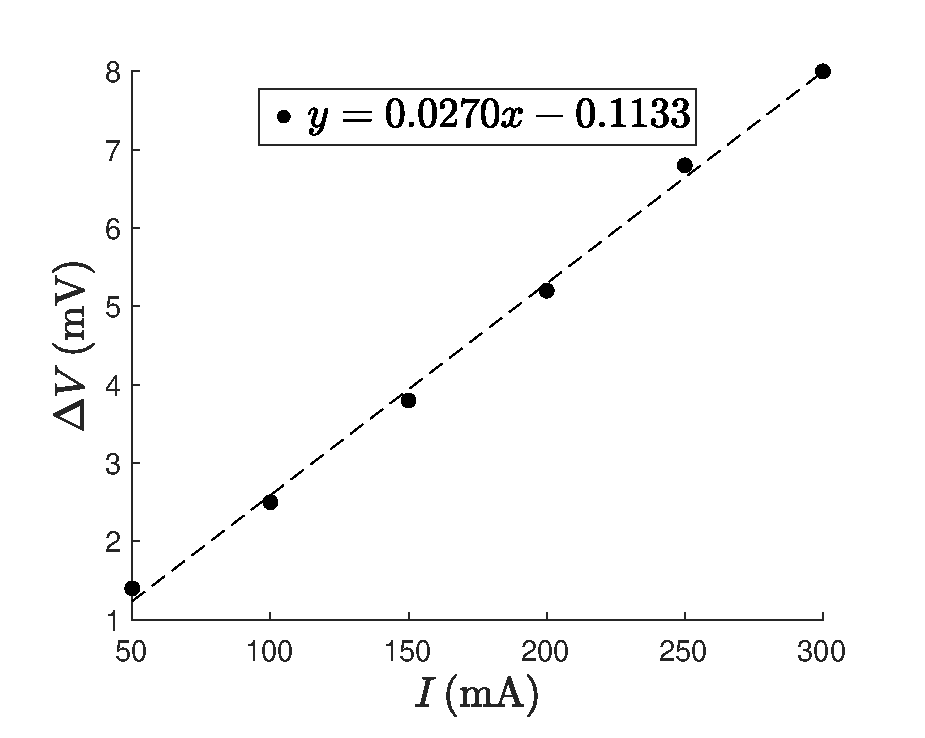
\includegraphics[width=0.8\columnwidth]{files/images/S1L1}
    \end{center}
    \caption{$\Delta V$ frente a $I$, cable $S = 1.5\,$mm$^2$ y $L = 1\,$m.}
    \label{fig:S1L1}
\end{figure}

\begin{figure}[h!]
    \begin{center}
        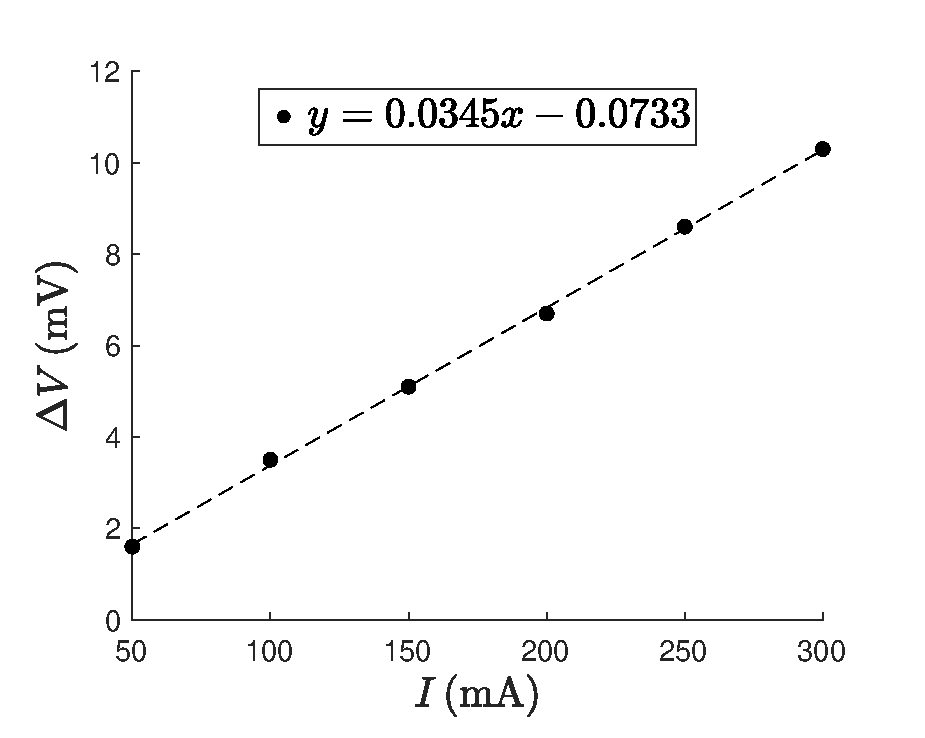
\includegraphics[width=0.8\columnwidth]{files/images/S1L2}
    \end{center}
    \caption{$\Delta V$ frente a $I$, cable $S = 1.5\,$mm$^2$ y $L = 1.5\,$m.}
    \label{fig:S1L2}
\end{figure}

\begin{figure}[h!]
    \begin{center}
        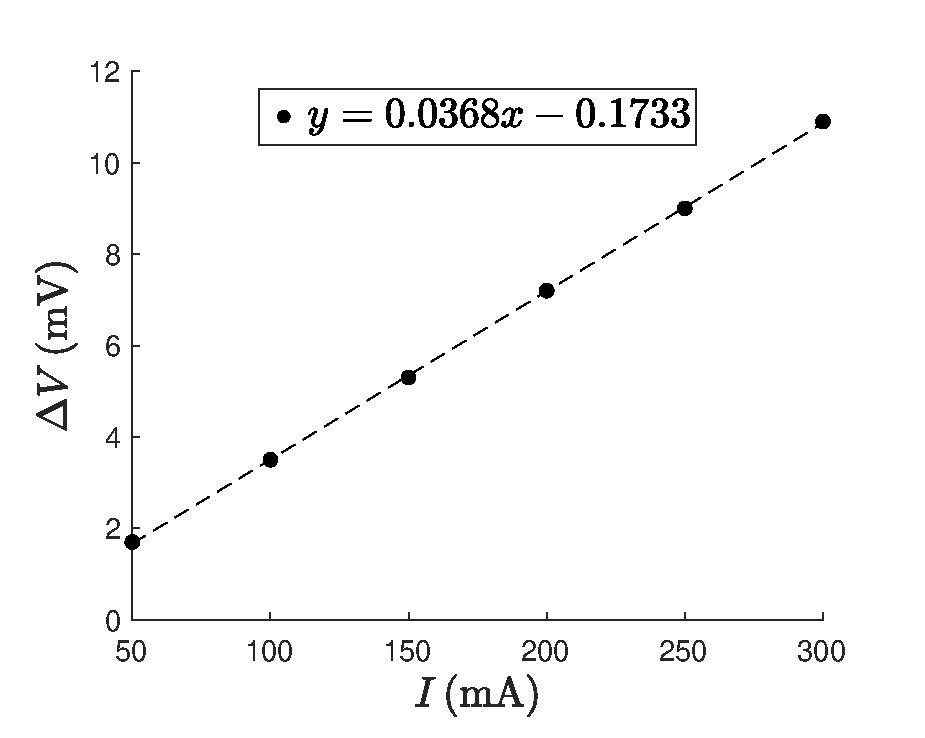
\includegraphics[width=0.8\columnwidth]{files/images/S1L3}
    \end{center}
    \caption{$\Delta V$ frente a $I$, cable $S = 1.5\,$mm$^2$ y $L = 2\,$m.}
    \label{fig:S1L3}
\end{figure}

\begin{figure}[h!]
    \begin{center}
        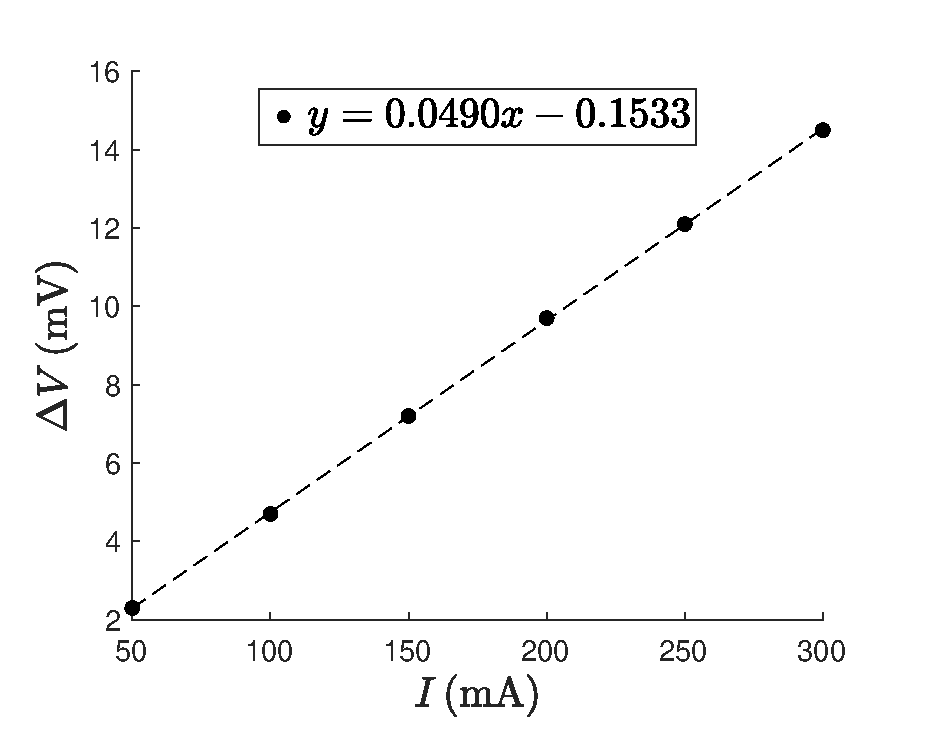
\includegraphics[width=0.8\columnwidth]{files/images/S2L1}
    \end{center}
    \caption{$\Delta V$ frente a $I$, cable $S = 0.5\,$mm$^2$ y $L = 1\,$m.}
    \label{fig:S2L1}
\end{figure}

\begin{figure}[h!]
    \begin{center}
        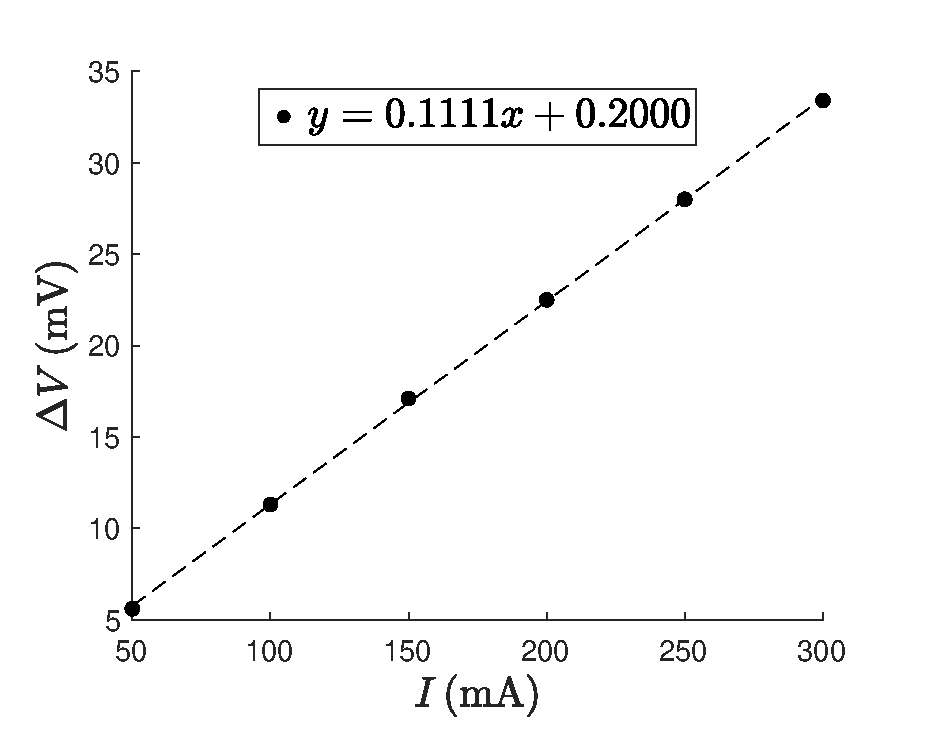
\includegraphics[width=0.8\columnwidth]{files/images/S2L2}
    \end{center}
    \caption{$\Delta V$ frente a $I$, cable $S = 0.5\,$mm$^2$ y $L = 1.5\,$m.}
    \label{fig:S2L2}
\end{figure}

\begin{figure}[h!]
    \begin{center}
        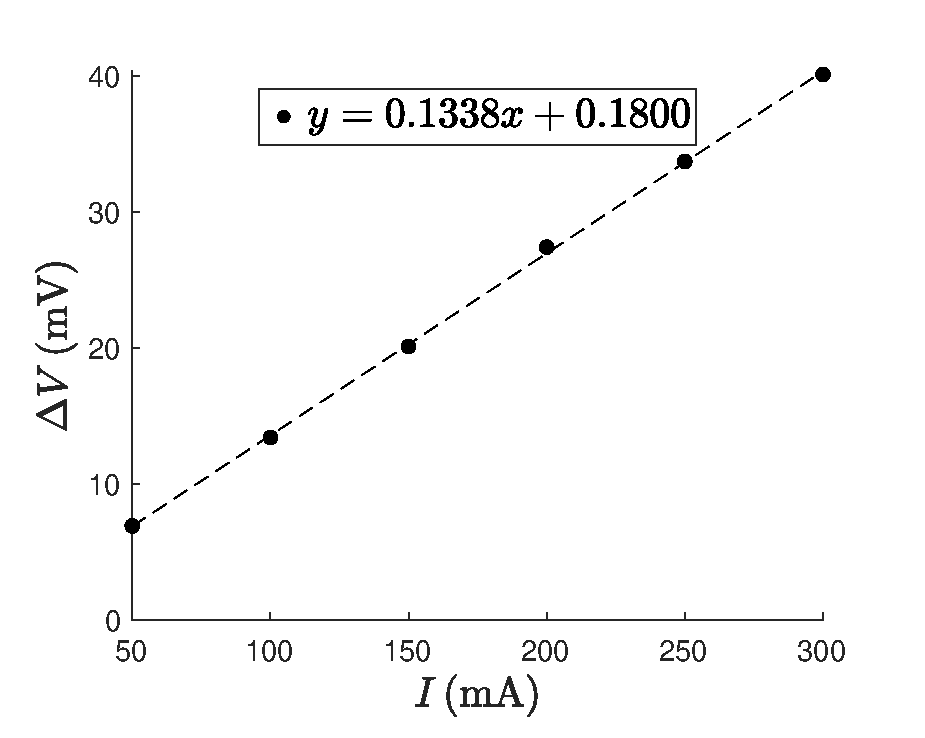
\includegraphics[width=0.8\columnwidth]{files/images/S2L3}
    \end{center}
    \caption{$\Delta V$ frente a $I$, cable $S = 0.5\,$mm$^2$ y $L = 2\,$m.}
    \label{fig:S2L3}
\end{figure}

\begin{figure}[h!]
    \begin{center}
        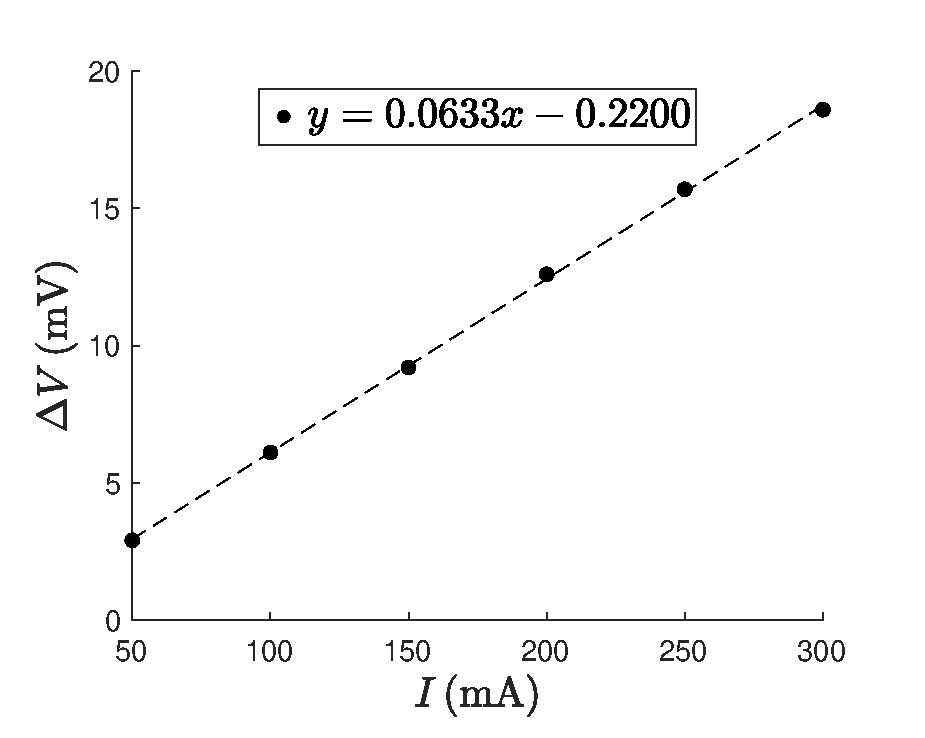
\includegraphics[width=0.8\columnwidth]{files/images/S3L1}
    \end{center}
    \caption{$\Delta V$ frente a $I$, cable $S = 0.325\,$mm$^2$ y $L = 1\,$m.}
    \label{fig:S3L1}
\end{figure}

\begin{figure}[h!]
    \begin{center}
        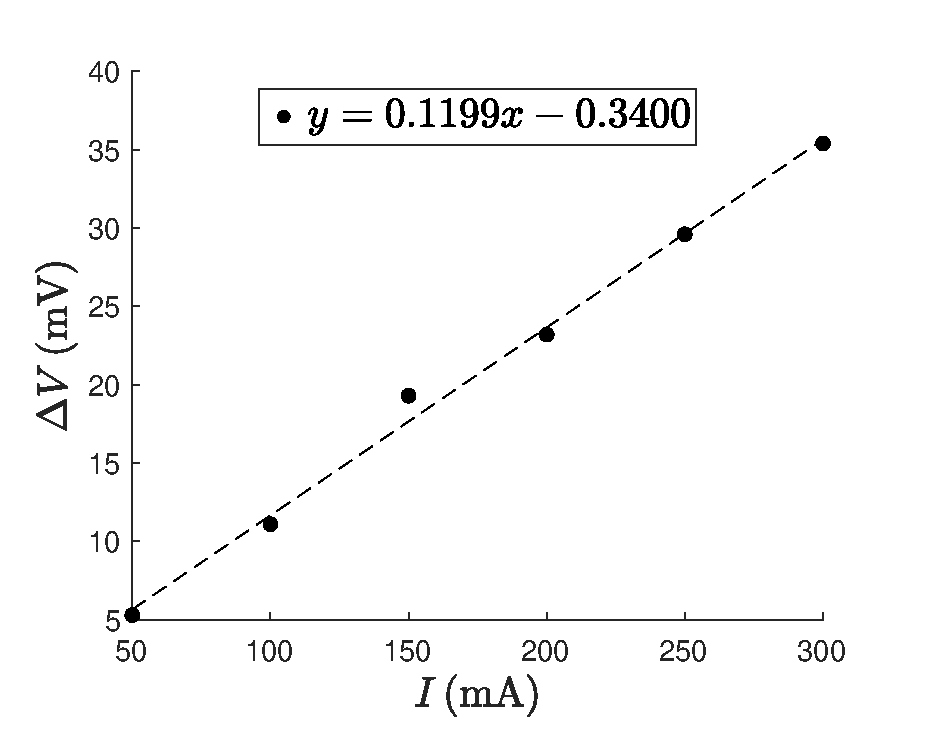
\includegraphics[width=0.8\columnwidth]{files/images/S3L2}
    \end{center}
    \caption{$\Delta V$ frente a $I$, cable $S = 0.32\,$mm$^2$ y $L = 1.5\,$m.}
    \label{fig:S3L2}
\end{figure}

\begin{figure}[h!]
    \begin{center}
        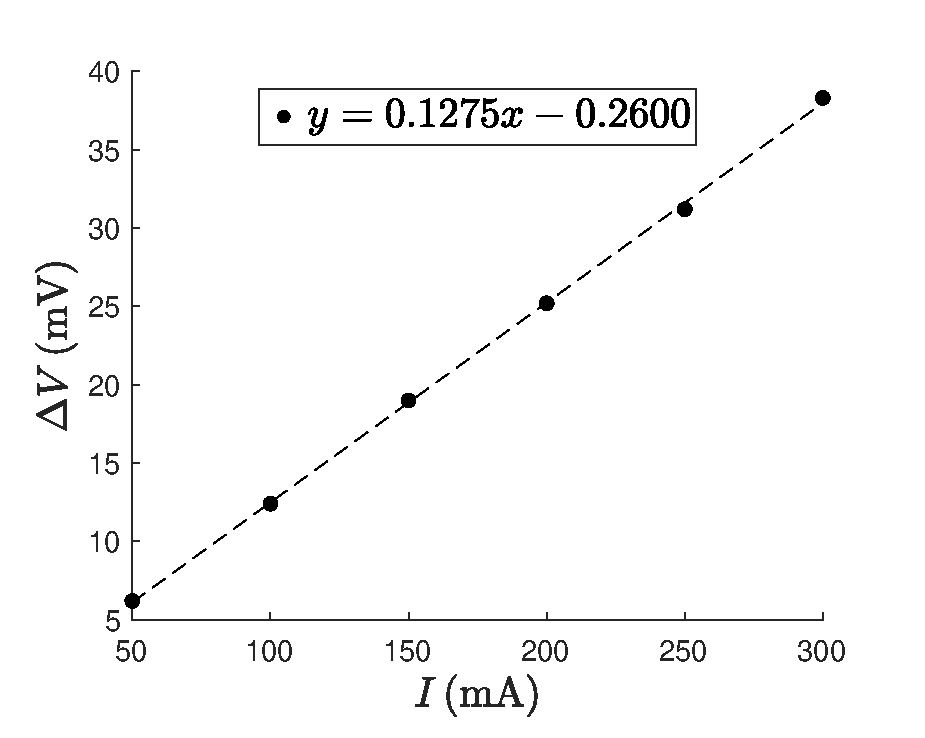
\includegraphics[width=0.8\columnwidth]{files/images/S3L3}
    \end{center}
    \caption{$\Delta V$ frente a $I$, cable $S = 0.32\,$mm$^2$ y $L = 2\,$m.}
    \label{fig:S3L3}
\end{figure}

\FloatBarrier

La ordenada en el origen que se obtiene en el ajuste de los datos es el valor que corresponder�a a
la diferencia de potencial $\Delta V$ para una intensidad de corriente $I$ nula.

Idealmente, el valor de la ordenada en el origen deber�a ser 0.
El que no lo sea indica que en nuestras mediciones experimentales hemos
introducido un error.

Adem�s, la pendiente de las rectas es distinta en cada caso
porque la resistencia de cada cable var�a con la longitud $L$ y tambi�n con la secci�n $S$, seg�n la expresi�n~\ref{eq:ressitividad}.

\subsection{}

La tabla~\ref{tab:R2} recoge los valores de la resistencia $R$ (en m$\Omega$) de cada serie en funci�n de la longitud $L$ y la secci�n $S$ de cada cable.

\begin{table}[h!]
    \caption{Resistencia de cada conductor seg�n su longitud $L$ y secci�n $S$.}
    \label{tab:R2}
    \begin{centering}
        \small
        \begin{tabular}{|P{18px}|P{52px}|P{52px}|P{56px}|}
            \hline
            & $S = 1.5\,$mm$^2$     & $S = 0.5\,$mm$^2$     & $S = 0.32\,$mm$^2$    \\
            \hline
            $L\,$(m) & $R\,(\text{m}\Omega)$ & $R\,(\text{m}\Omega)$ & $R\,(\text{m}\Omega)$ \\
            \hline
            $1$      & $27.0 \pm 0.7$        & $49.0 \pm 0.2$        & $63.3 \pm 0.6$        \\
            $1.5$    & $34.5 \pm 0.5$        & $111.1 \pm 0.8$       & $120 \pm 4$           \\
            $2$      & $36.8 \pm 0.2$        & $133.8 \pm 1.3$       & $127.5 \pm 1.3$       \\
            \hline
        \end{tabular}
    \end{centering}
\end{table}

Estos valores son la pendiente de las rectas de las gr�ficas de la secci�n~\ref{subsec:analisis1}.

El error mostrado es el error est�ndar de la regresi�n lineal.

\subsection{}

Las figuras~\ref{fig:RL1},~\ref{fig:RL2} y~\ref{fig:RL3} muestran la representaci�n de $R$ frente a $L$
para cada cable.

\begin{figure}[h!]
    \begin{center}
        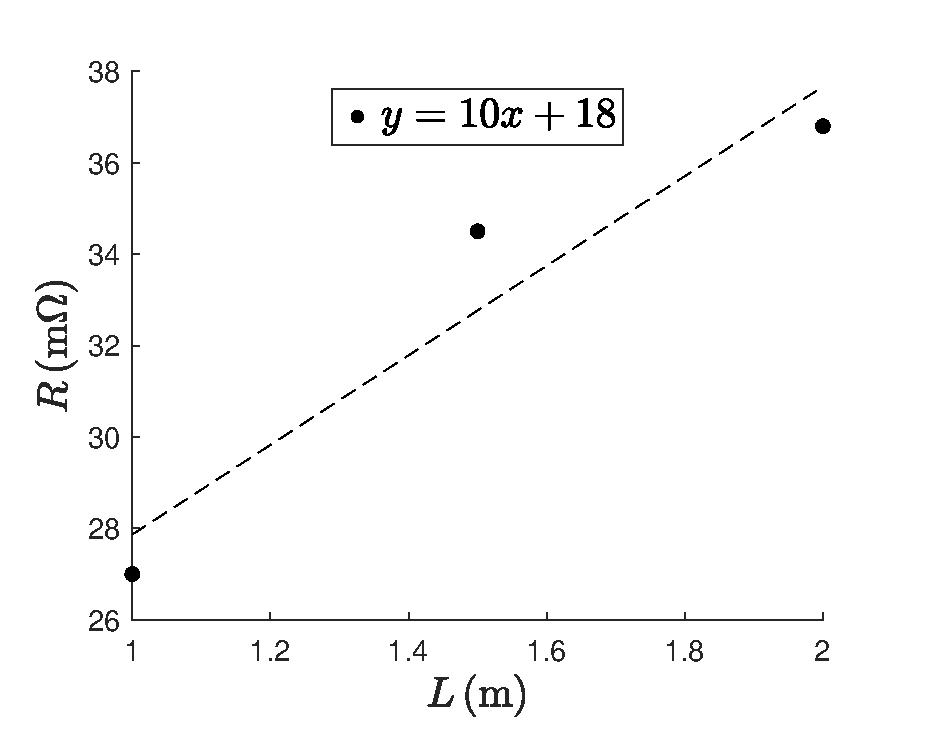
\includegraphics[width=0.8\columnwidth]{files/images/RL1}
    \end{center}
    \caption{$R$ frente a $L$, cable $S = 1.5\,$mm$^2$.}
    \label{fig:RL1}
\end{figure}

\FloatBarrier

La pendiente $m$ y la ordenada en el origen $b$ de la regresi�n lineal de la figura~\ref{fig:RL1} son:
\begin{align*}
    m & = (10 \pm 3)\,\Omega / \text{m}\\
    b & = (18 \pm 5)\,\Omega / \text{m}
\end{align*}

\begin{figure}[h!]
    \begin{center}
        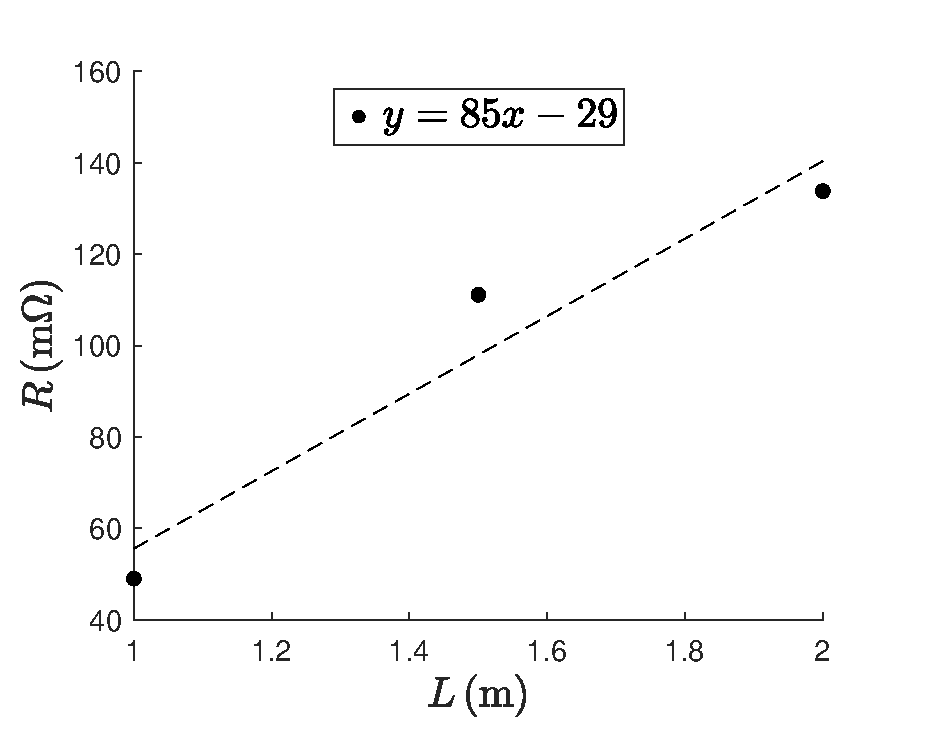
\includegraphics[width=0.8\columnwidth]{files/images/RL2}
    \end{center}
    \caption{$R$ frente a $L$, cable $S = 0.5\,$mm$^2$.}
    \label{fig:RL2}
\end{figure}

\FloatBarrier

La pendiente $m$ y la ordenada en el origen $b$ de la regresi�n lineal de la figura~\ref{fig:RL2} son:
\begin{align*}
    m & = (84 \pm 20)\,\Omega / \text{m}\\
    b & = (-30 \pm 40)\,\Omega / \text{m}
\end{align*}

\begin{figure}[h!]
    \begin{center}
        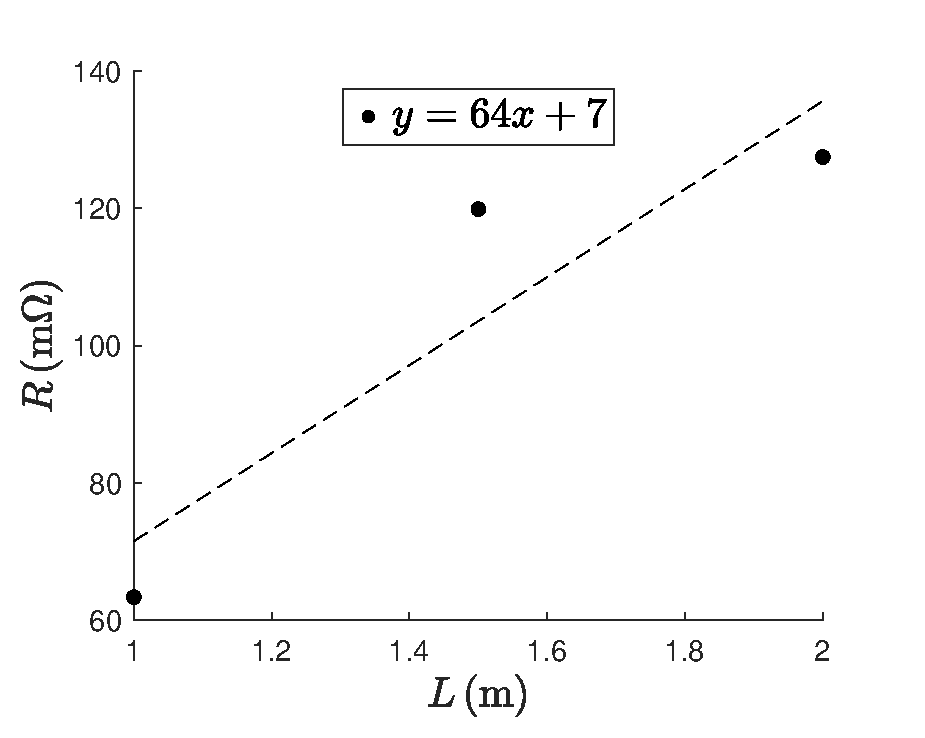
\includegraphics[width=0.8\columnwidth]{files/images/RL3}
    \end{center}
    \caption{$R$ frente a $L$, cable $S = 0.32\,$mm$^2$.}
    \label{fig:RL3}
\end{figure}

\FloatBarrier
La pendiente $m$ y la ordenada en el origen $b$ de la regresi�n lineal de la figura~\ref{fig:RL3} son:
\begin{align*}
    m & = (60 \pm 30)\,\Omega / \text{m}\\
    b & = (10 \pm 40)\,\Omega / \text{m}
\end{align*}

La pendiente de cada recta es la resistencia $R$ del cable por unidad de longitud $L$.
Existen 3 rectas porque existen 3 cables con secci�n transversal distinta.





